\documentclass{article}
\usepackage[utf8]{inputenc}
\usepackage[T1]{fontenc}
\usepackage[catalan]{babel}
\usepackage[vmargin=3cm]{geometry}
\usepackage{lastpage}
\usepackage{lipsum}
\usepackage{graphicx}
\usepackage{parskip}
\usepackage[hyphens]{url}
\usepackage{hyperref}
\usepackage{caption}
\usepackage{listings}
\usepackage[section]{placeins}

\usepackage{silence}
\WarningFilter{latex}{You have requested package}
\usepackage{../../common/listings-rust}

\Urlmuskip=0mu plus 2mu

\hypersetup{
    colorlinks=true,
    linkcolor=black,
    urlcolor=blue,
    citecolor=red,
}

\graphicspath{ {img/} }

\lstnewenvironment{code}[1][]{
   \noindent
   \lstset{
        language=Rust,
        style=colouredRust,
        inputencoding=latin1
    }
}{}

\begin{document}
\begin{titlepage}
	\newcommand{\HRule}{\rule{\linewidth}{0.4mm}} % Defines a new command for horizontal lines, change thickness here
	
	\center

    \vspace*{25px}
    % == Headings ==
	
	\textsc{\LARGE Universitat Autònoma de Barcelona}\\[1.5cm]

	\textsc{\Large Treball de Fi de Grau}\\[0.5cm]
	
	\textsc{\Large Informe de progrés II}\\[0.5cm]
	
	\HRule\\[0.4cm]
	
	{\LARGE\bfseries Disseny i implementació d'un llenguatge de programació amb LLVM}\\[0.4cm]
	
	\HRule\\[1.5cm]
	
	% == Author ==
	
	\begin{minipage}{0.5\textwidth}
		\begin{flushleft}
			\large
			\textit{Autor}\\
			\textsc{Josep Maria Domingo Catafal}
		\end{flushleft}
	\end{minipage}
	~
	\begin{minipage}{0.4\textwidth}
		\begin{flushright}
			\large
			\textit{Tutor}\\
			\textsc{Javier Sánchez Pujadas}
		\end{flushright}
	\end{minipage}
	
	% == Date == 

	\vfill\vfill\vfill % Position the date 3/4 down the remaining page
	
	{\large\today} % Date, change the \today to a set date if you want to be precise

	\vfill % Push the date up 1/4 Of the remaining page
\end{titlepage}

% --------------------------------------
% Table of contents
% --------------------------------------
\tableofcontents
\newpage

% --------------------------------------
% Body
% --------------------------------------

\section{Control de qualitat}
Els tests automatitzats són una part important del desenvolupament de
programari, ja que ajuda a assegurar la qualitat i la fiabilitat del codi. Ens
permet detectar i arreglar errors que poder no hauríem detectat provant-ho a mà.
A més a més, a mesura que el projecte es va fent gran, és inviable provar-ho tot
de forma manual.

Hi ha diferents tipus de tests automatitzats que es poden implementar. Els tests
unitaris són un tipus de test que es centren en unitats individuals de codi, com
ara funcions o mètodes. En el meu cas, he implementat tests unitaris pel parser,
per així verificar que l'arbre sintàctic que es genera és correcte. 

Tot i això, és poc pràctic implementar aquests tests, ja que has de tenir
l'arbre correcte, "hardcoded" en el test per comprovar que el resultat sigui
aquest, i en arbres més grans és poc viable. Per aquest motiu la majoria de
tests que he implementat són tests d'integració.

Els tests d'integració són un altre tipus de test automatitzat que se centren en
com diferents unitats de codi treballen juntes. La forma en la qual els he 
implementat és escrivint programes en el llenguatge desenvolupat, compilant-los 
i executant-los i comprovant que el resultat és l'esperat. Per exemple pels 
arrays hi ha un petit programa que crea un array, el passa com a paràmetre a una
funció i fa print dels seus elements. Aleshores el test comprovaria que els 
valors printats siguin els de l'array. I després faríem un altre test que 
accedeix a un índex de l'array que no existeix i comprovaríem que el programa 
falla amb un error 'index out of bounds'.

Aquests tests són importants perquè ajuden a assegurar que tots els components
del llenguatge funcionen correctament entre ells.

\subsection{Integració amb el control de versions del codi font}

Com vam comentar a l'informe anterior per al control de versions del codi font
s'està utilitzant Git i GitHub (\url{https://github.com/josepmdc/craft}).
Respecte a l'anterior informe ha canviat una cosa, i és que com que ara disposem
de tests automatitzats, podem fer ús d'una funcionalitat de GitHub que s'anomena
GitHub Actions. El que ens permeten fer les Actions, és executar en els
servidors de GitHub alguna tasca, depenent d'alguns events com ara quan es fa un
commit a master. Per exemple, jo he configurat que cada vegada que s'obri una
pull request i cada vegada que es faci un commit a master, que s'executin tots
els tests del projecte. D'aquesta manera cada vegada que es vulguin incorporar
canvis a master, t'assegures que no s'ha trencat res i tot funciona amb
normalitat. A part dels tests, he afegit 3 tasques més que s'executen en els 
dos casos que hem comentat anteriorment. Així que tenim les 4 tasques següents:

\begin{itemize}
    \item Executa tots els tests, tant d'integració com unitaris.
    \item Comprova que el projecte compili correctament.
    \item Comprova que el codi estigui formatat seguint la guia d'estil.
    \item Executa clippy, un linter que ve incorporat amb el llenguatge de Rust 
        i que et permet millorar el codi a través de suggeriments i t'informa de
        possibles bugs.
\end{itemize}

En cas que alguna d'aquestes quatre tasques falli o retorni algun warning, 
no es podrà fer merge fins que es resolguin els problemes.

Per configurar les Actions és força senzill, ja que es fa a través de uns arxius
de configuració en format YAML, en el qual l'hi especifiques el sistema operatiu
que vols fer servir així com totes les tasques que vols que executi. Hi ha 
algunes Actions que ha desenvolupat la comunitat i que tu simplement les 
referències a la teva configuració indicant que les executi. Per exemple per la
tasca de executar els tests la configuració seria així:

\begin{verbatim}
on:
  pull_request:
  push:
    branches: master

name: Continuous integration

jobs:
  test:
    name: Test Suite
    runs-on: ubuntu-latest
    steps:
      - uses: actions/checkout@v2
      - uses: actions-rs/toolchain@v1
        with:
          profile: minimal
          toolchain: stable
          override: true
      - uses: actions-rs/cargo@v1
        with:
          command: test
\end{verbatim}

El que ens indica la configuració anterior és que quan s'obri una pull request o
es faci un push a master, s'executin els jobs que hi ha indicats. El job de test
indica que s'executarà en l'última versió d'Ubuntu i que té tres passos (steps).
El primer fa servir una action que es diu checkout, que el que fa és
descarregar-se el teu repositori en el servidor. El segon pas fa servir una
action que es diu toolchain, que instal·la totes els eines necessaries per
compilar Rust. I finalment l'ultim fa servir l'action de cargo. Cargo és l'eina
de Rust que es fa servir per compilar (\texttt{cargo build}), executar els tests
(\texttt{cargo test}), o descarregar llibreries, entre d'altres. Amb aquesta
action l'hi estem indicant que executi \texttt{cargo test}.

Per la resta de tasques que em comentat com ara la de clippy, simplement hem 
d'afegir un altre job a l'arxiu de configuració, de manera similar a com hem 
fet amb el de test.

\begin{figure}[!htb]
    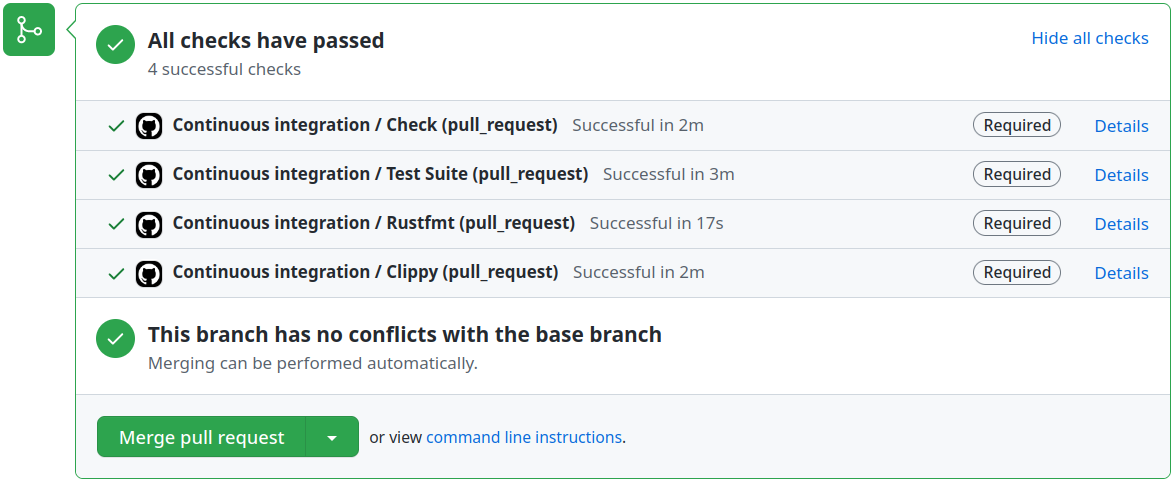
\includegraphics[width=\linewidth]{ci-pr-success.png}
    \centering
    \captionsetup{justification=centering}
    \caption{Pull Request on els checks han passat tots i que per tant es pot fer merge}
\end{figure}

\begin{figure}[!htb]
    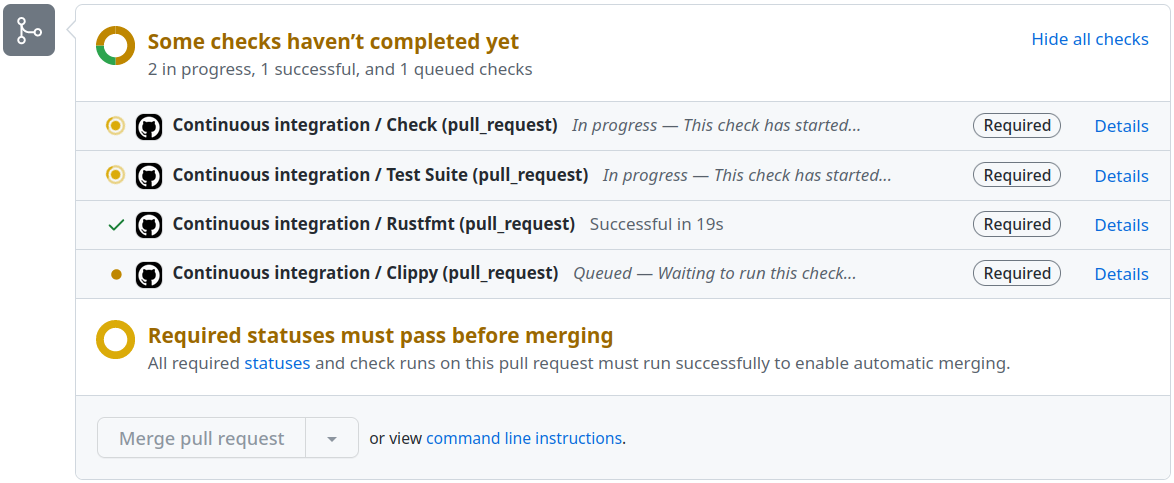
\includegraphics[width=\linewidth]{ci-pr-inprogress.png}
    \centering
    \captionsetup{justification=centering}
    \caption{Pull Request on els checks encara no s'han executat i que per tant no es pot fer merge}
\end{figure}

\begin{figure}[!htb]
    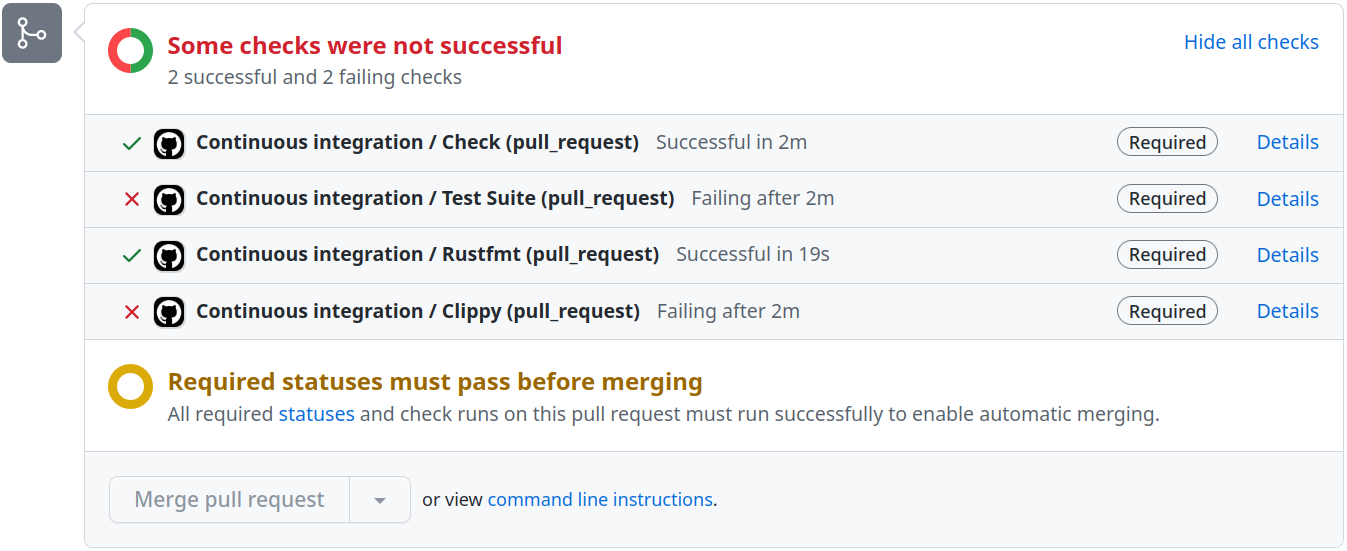
\includegraphics[width=\linewidth]{ci-pr-fail.png}
    \centering
    \captionsetup{justification=centering}
    \caption{Pull Request on els checks han fallat i que per tant no es pot fer merge}
\end{figure}

\section{Seguiment de la planificació}

Si recordem, a l'inici del treball vam definir quines eren les èpiques que
conformarien el projecte i en quin moment es desenvoluparien. A hores d'ara
aquestes èpiques segueixen més o menys com s'havien plantejat al seu moment,
però amb algun canvi pel que fa al moment en el qual s'han desenvolupat (alguna
ha durat més de l'esperat). També s'ha creat una nova èpica per albergar tots
els bugs i tasques de manteniment i millora del projecte que van apareixent a
mesura que va avançant. 

A continuació mirarem aquestes èpiques, una per una, per veure quin és el seu
estat, i, per les que ja s'han completat, donar una mica més de detall de què
han aportat al projecte i com s'han desenvolupat a un nivell més tècnic.

\subsection{Implementació mínima de l'especificació}
\textit{\textbf{Completada}: 13/09/2022 - 16/10/2022} (5 esprints)

Aquesta tasca ja va ser completada en l'informe anterior.

\subsection{Declaració de tipus}
\textit{\textbf{Completada}: 17/10/2022 - 6/11/2022} (3 esprints)

Aquesta tasca ja va ser completada en l'informe anterior.

\subsection{Collections}
\textit{\textbf{Completada}: 31/10/2022 - 20/11/2022*} (3 esprints)

\subsection{Mecanisme de gestió d'errors}
\textit{\textbf{Cancel·lada}: 21/11/2022 - 11/12/2022} (3 esprints)

Aquesta èpica ha sigut cancel·lada principalment perquè començaven a haver-hi 
bastants bugs al programa i vaig decidir que era més important solucionar-los
i tenir una base sòlida que seguir afegint funcionalitats. L'he cancel·lat en 
comptes d'aplaçar-la, ja que prefereixo fer l'èpica de Syntactic Sugar.

\subsection{Syntactic sugar}
\textit{\textbf{Planificada}: 12/12/2022 - 02/01/2023} (3 esprints)

Implementació de "Syntactic sugar", per tal de simplificar operacions que
s'utilitzen freqüentment. Inclou bucles for in, match (similar a un switch),
list comprehension, etc.

\subsection{Suport per programació d'estil funcional}
\textit{\textbf{Cancel·lada}: 03/01/2023 - 23/01/2023} (3 esprints)

Pel mateix motiu que l'èpica de gestió d'errors, he decidit cancel·lar aquesta
èpica. Les tres setmanes en les quals s'havia de fer aquesta èpica seran les
tres últimes setmanes i m'estimo més dedicar aquests temps a millorar el que ja
tingui fent i estabilitzar-ho tot.

\subsection{Deute tècnic}
\textit{\textbf{En progrés}: Termini indefinit} ($\infty$ esprints)

Com hem comentat, hi ha diversos bugs que han anat apareixent i per tant, el
temps que estava destinat a l'èpica de gestió d'errors s'ha destinat a aquesta
èpica. A continuació veurem alguns dels bugs que s'han solucionat (els més
greus o que comporten més feina d'arreglar).

\subsubsection{Taula de símbols}

La taula de símbols que tenia fins ara no funcionava del tot bé i estava donant
problemes. Així que en vaig implementar una de nova, aquest cop fent-ho bé.

Vaig crear una classe amb diferents funcions per tal de poder crear o eliminar
un context nou quan fes falta. Consisteix simplement d'un vector de HashMaps,
que actua com a pila. Cada HashMap és un context diferent. La classe conté les
següents funcions:

\begin{itemize}
    \item \texttt{\textbf{new\_context}}: Afegeix un nou HashMap a la pila.
    \item \texttt{\textbf{pop\_context}}: Treu l'últim HashMap de la pila.
    \item \texttt{\textbf{insert}}: Afegeix una nova variable a la taula de dalt
    de tot de la pila.
    \item \texttt{\textbf{get}}: Busca una variable en les taules que hi ha a la
    pila. En cas de no trobar-la, retorna un error (UndeclaredVariableOrOutOfScope)
\end{itemize}

Amb aquestes funcions en tenim prou per tenir una taula de símbols funcional. Es
crea un context nou cada vegada que es crea un bloc (s'obre amb '\{') i
s'elimina quan s'acaba el bloc (es tanca amb '\}').

\subsubsection{Blocs sempre havien de retornar un valor}

Una de les característiques clau del llenguatge és que és un llenguatge basat en
expressions, el que significa que la majoria de les declaracions del llenguatge
retornen un valor. Un exemple són els blocs de codi (conjunt de sentències dins
de \{\}), els quals si l'última sentència del bloc no porta punt i coma, aquesta
serà una expressió i per tant el seu valor serà retornat. Per exemple el següent
bloc retorna el resultat de 2 + 2:

\begin{code}
    let four = {
        2 + 2
    };
\end{code}

El problema és que tal com s'havien implementat els blocs, sempre havien de
retornar un valor, encara que no volguessis retornar res. Aleshores, en casos
com un bucle while, per exemple, que està format per un bloc, no té massa sentit
voler retornar un valor. Per tant era una cosa que havia de ser solucionada.

\subsubsection{Error en cridar funcions que no retornaven valor}

Com hem comentat abans, el llenguatge està orientat a expressions i per tant
pràcticament tot pot retornar un valor. Però a vegades no volem que en retorni
cap. Igual que amb els blocs, hi havia un problema al cridar funcions que no
retornaven cap valor (void), ja que tal com estava estructurat el compilador,
esperava que una expressió \textbf{sempre} retornes un valor. I com que una
crida a una funció és una expressió, quan cridàvem una funció que no retorna
valor fallava. Per solucionar aquest problema, el que s'ha fet és que les
funcions void, també retornin un valor, l'únic que és un valor buit, que no té
res, ni mida ni tipus ni valor, com una tupla buida.

\newpage
\renewcommand\refname{Bibliografia}
\begin{thebibliography}{9}

\bibitem{llvmtut} \textit{LLVM Kaleidoscope Tutorial: Implementing a Language with LLVM}. Accedit el 25 d'octubre, 2022, des de \url{https://llvm.org/docs/tutorial}
\bibitem{llvm4plc} Rathi, M. \textit{A complete guide to LLVM for programming language creators}. Mukuls Blogs. Accedit el 2 de Novembre, 2022, des de \\\url{https://mukulrathi.com/create-your-own-programming-language/llvm-ir-cpp-api-tutorial}
\bibitem{ci} Nystrom, R. \textit{Crafting Interpreters}. Publicat Juliol, 2021. ISBN 0990582930.
\bibitem{mhlctllvm} \textit{Mapping High Level Constructs to LLVM IR}. Accedit el 20 d'octubre, 2022 des de \\\url{https://mapping-high-level-constructs-to-llvm-ir.readthedocs.io/en/latest/README.html}
\bibitem{inkwell} \textit{Inkwell Documentation}. Accedit el 4 d'octubre, 2022 des de \\\url{https://thedan64.github.io/inkwell/inkwell/index.html}
\bibitem{compilergo} Ball, T. \textit{Writing A Compiler In Go}. Publicat Agost, 2018. ISBN 398201610X.

\end{thebibliography}
\end{document}
